\documentclass[twoside]{book}

% Packages required by doxygen
\usepackage{calc}
\usepackage{doxygen}
\usepackage{graphicx}
\usepackage[utf8]{inputenc}
\usepackage{makeidx}
\usepackage{multicol}
\usepackage{multirow}
\usepackage{textcomp}
\usepackage[table]{xcolor}

% Font selection
\usepackage[T1]{fontenc}
\usepackage{mathptmx}
\usepackage[scaled=.90]{helvet}
\usepackage{courier}
\usepackage{amssymb}
\usepackage{sectsty}
\renewcommand{\familydefault}{\sfdefault}
\allsectionsfont{%
  \fontseries{bc}\selectfont%
  \color{darkgray}%
}
\renewcommand{\DoxyLabelFont}{%
  \fontseries{bc}\selectfont%
  \color{darkgray}%
}

% Page & text layout
\usepackage{geometry}
\geometry{%
  a4paper,%
  top=2.5cm,%
  bottom=2.5cm,%
  left=2.5cm,%
  right=2.5cm%
}
\tolerance=750
\hfuzz=15pt
\hbadness=750
\setlength{\emergencystretch}{15pt}
\setlength{\parindent}{0cm}
\setlength{\parskip}{0.2cm}
\makeatletter
\renewcommand{\paragraph}{%
  \@startsection{paragraph}{4}{0ex}{-1.0ex}{1.0ex}{%
    \normalfont\normalsize\bfseries\SS@parafont%
  }%
}
\renewcommand{\subparagraph}{%
  \@startsection{subparagraph}{5}{0ex}{-1.0ex}{1.0ex}{%
    \normalfont\normalsize\bfseries\SS@subparafont%
  }%
}
\makeatother

% Headers & footers
\usepackage{fancyhdr}
\pagestyle{fancyplain}
\fancyhead[LE]{\fancyplain{}{\bfseries\thepage}}
\fancyhead[CE]{\fancyplain{}{}}
\fancyhead[RE]{\fancyplain{}{\bfseries\leftmark}}
\fancyhead[LO]{\fancyplain{}{\bfseries\rightmark}}
\fancyhead[CO]{\fancyplain{}{}}
\fancyhead[RO]{\fancyplain{}{\bfseries\thepage}}
\fancyfoot[LE]{\fancyplain{}{}}
\fancyfoot[CE]{\fancyplain{}{}}
\fancyfoot[RE]{\fancyplain{}{\bfseries\scriptsize Generated on Sat Jun 14 2014 16\-:44\-:50 for xpathtool by Doxygen }}
\fancyfoot[LO]{\fancyplain{}{\bfseries\scriptsize Generated on Sat Jun 14 2014 16\-:44\-:50 for xpathtool by Doxygen }}
\fancyfoot[CO]{\fancyplain{}{}}
\fancyfoot[RO]{\fancyplain{}{}}
\renewcommand{\footrulewidth}{0.4pt}
\renewcommand{\chaptermark}[1]{%
  \markboth{#1}{}%
}
\renewcommand{\sectionmark}[1]{%
  \markright{\thesection\ #1}%
}

% Indices & bibliography
\usepackage{natbib}
\usepackage[titles]{tocloft}
\setcounter{tocdepth}{3}
\setcounter{secnumdepth}{5}
\makeindex

% Custom commands
\newcommand{\clearemptydoublepage}{%
  \newpage{\pagestyle{empty}\cleardoublepage}%
}


%===== C O N T E N T S =====

\begin{document}

% Titlepage & ToC
\pagenumbering{roman}
\begin{titlepage}
\vspace*{7cm}
\begin{center}%
{\Large xpathtool \\[1ex]\large 1.\-0-\/13 }\\
\vspace*{1cm}
{\large Generated by Doxygen 1.8.6}\\
\vspace*{0.5cm}
{\small Sat Jun 14 2014 16:44:50}\\
\end{center}
\end{titlepage}
\clearemptydoublepage
\tableofcontents
\clearemptydoublepage
\pagenumbering{arabic}

%--- Begin generated contents ---
\chapter{Java\-Doc A\-P\-I Markup for xpathtool}
\label{index}\section*{xpathtool }

Simple get/set tools for X\+Path-\/based X\+M\+L manipulation

This content started as slightly-\/modified xmlsoft.\+org example code, therefore is ({\tt http\+://xmlsoft.\+org/\+F\+A\+Q.\+html}) M\+I\+T-\/\+Licensed. The Java code is all new, but is intended to provide the same functionality in a pure-\/java environment, so remains abstractly \char`\"{}derived\char`\"{}. 
\chapter{R\-E\-A\-D\-M\-E}
\label{md_htdocs_README}
\input{md_htdocs_README}
\chapter{Hierarchical Index}
\section{Class Hierarchy}
This inheritance list is sorted roughly, but not completely, alphabetically\+:\begin{DoxyCompactList}
\item Exception\item \contentsline{section}{No\+Document\+Exception}{\pageref{classorg_1_1smallfoot_1_1xpath_1_1NoDocumentException}}{}
\item \contentsline{section}{version}{\pageref{classorg_1_1smallfoot_1_1xpath_1_1version}}{}
\item \contentsline{section}{X\+Path\+Set}{\pageref{classorg_1_1smallfoot_1_1xpath_1_1XPathSet}}{}
\item \contentsline{section}{X\+Path\+Sub}{\pageref{classorg_1_1smallfoot_1_1xpath_1_1XPathSub}}{}
\item \contentsline{section}{X\+Path\+Tool}{\pageref{classorg_1_1smallfoot_1_1xpath_1_1XPathTool}}{}
\end{DoxyCompactList}

\chapter{Data Structure Index}
\section{Data Structures}
Here are the data structures with brief descriptions\-:\begin{DoxyCompactList}
\item\contentsline{section}{{\bf No\-Document\-Exception} }{\pageref{classorg_1_1smallfoot_1_1xpath_1_1NoDocumentException}}{}
\item\contentsline{section}{{\bf version} }{\pageref{classorg_1_1smallfoot_1_1xpath_1_1version}}{}
\item\contentsline{section}{{\bf X\-Path\-Set} \\*A driving class to interpret commandline arguments and pass them to the underlying \doxyref{X\-Path\-Tool}{p.}{classorg_1_1smallfoot_1_1xpath_1_1XPathTool} }{\pageref{classorg_1_1smallfoot_1_1xpath_1_1XPathSet}}{}
\item\contentsline{section}{{\bf X\-Path\-Sub} \\*A driving class to interpret commandline arguments and pass them to the underlying \doxyref{X\-Path\-Tool}{p.}{classorg_1_1smallfoot_1_1xpath_1_1XPathTool} }{\pageref{classorg_1_1smallfoot_1_1xpath_1_1XPathSub}}{}
\item\contentsline{section}{{\bf X\-Path\-Tool} \\*\doxyref{X\-Path\-Tool}{p.}{classorg_1_1smallfoot_1_1xpath_1_1XPathTool} is a relatively uncomplicated wrapper for an X\-Path action\-: it doesn't know what you're doing, and doesn't assume you'll do things in a specific order, but tries to stop you from making really silly errors like saving or searching an unloaded file }{\pageref{classorg_1_1smallfoot_1_1xpath_1_1XPathTool}}{}
\end{DoxyCompactList}

\chapter{Data Structure Documentation}
\section{No\-Document\-Exception Class Reference}
\label{classorg_1_1smallfoot_1_1xpath_1_1NoDocumentException}\index{No\-Document\-Exception@{No\-Document\-Exception}}


Inheritance diagram for No\-Document\-Exception\-:\nopagebreak
\begin{figure}[H]
\begin{center}
\leavevmode
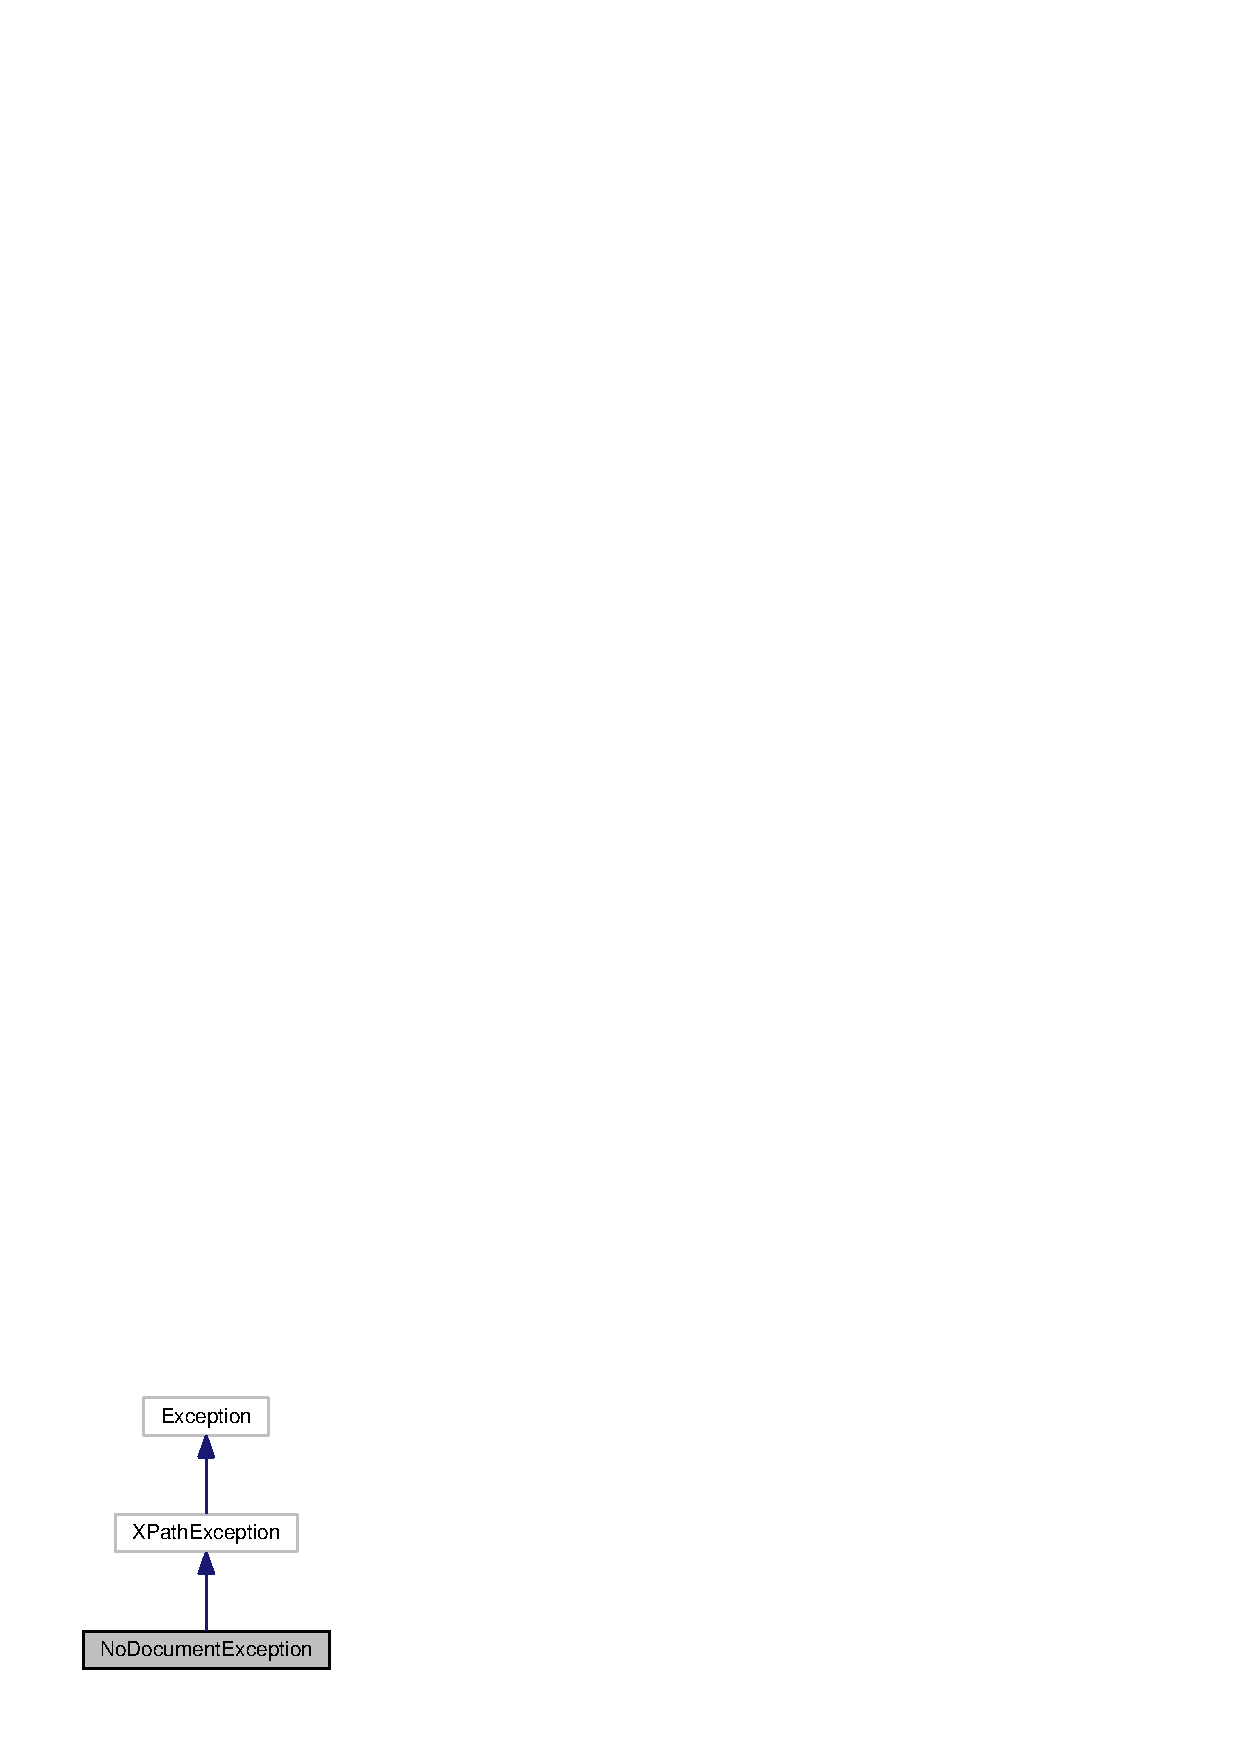
\includegraphics[width=162pt]{classorg_1_1smallfoot_1_1xpath_1_1NoDocumentException__inherit__graph}
\end{center}
\end{figure}


Collaboration diagram for No\-Document\-Exception\-:\nopagebreak
\begin{figure}[H]
\begin{center}
\leavevmode
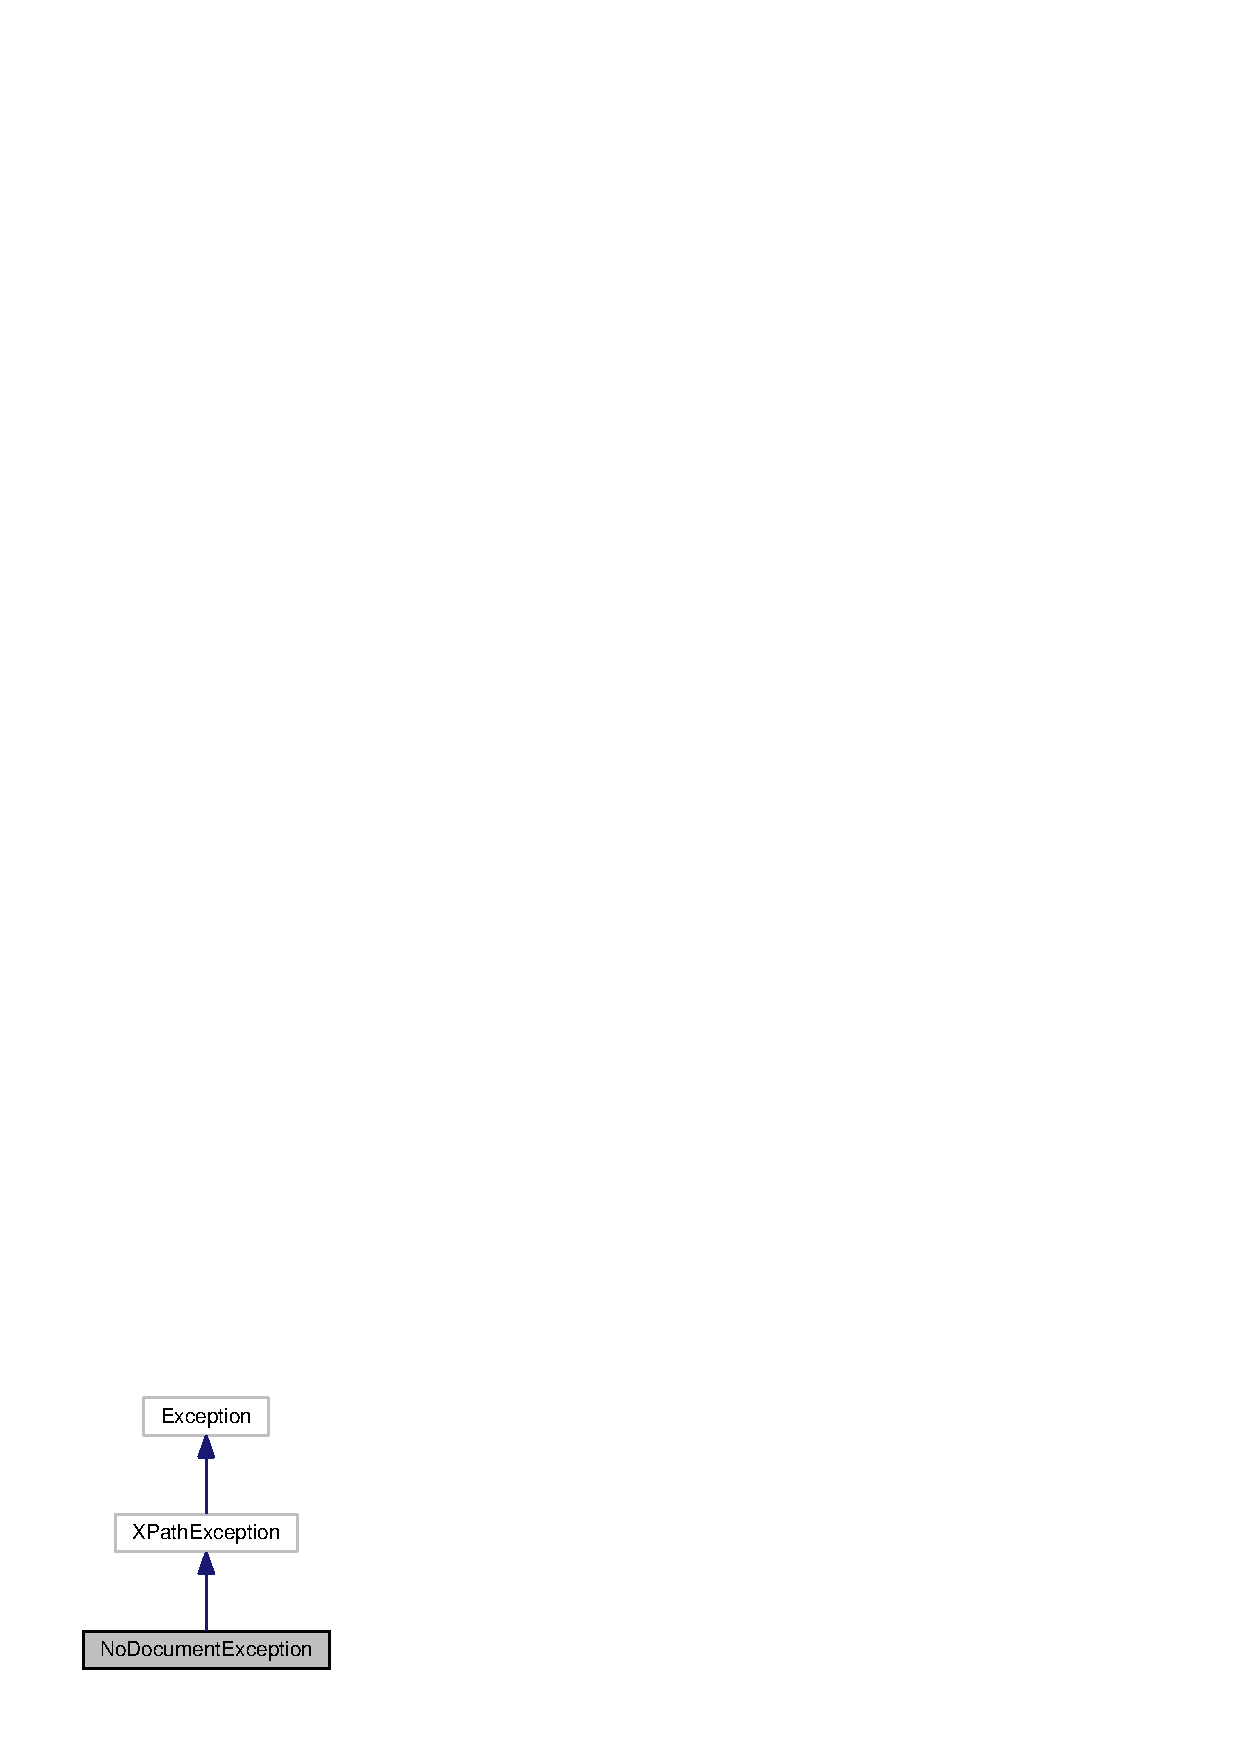
\includegraphics[width=162pt]{classorg_1_1smallfoot_1_1xpath_1_1NoDocumentException__coll__graph}
\end{center}
\end{figure}


\subsection{Detailed Description}


Definition at line 3 of file No\-Document\-Exception.\-java.



The documentation for this class was generated from the following file\-:\begin{DoxyCompactItemize}
\item 
java/No\-Document\-Exception.\-java\end{DoxyCompactItemize}

\section{version Class Reference}
\label{classorg_1_1smallfoot_1_1xpath_1_1version}\index{version@{version}}


version is used to allow a package that uses this package to be able to \char`\"{}ask\char`\"{} the jar file what version it is  


\subsection*{Static Public Member Functions}
\begin{DoxyCompactItemize}
\item 
static void {\bf main} (String arg[$\,$])
\begin{DoxyCompactList}\small\item\em returns the version of the class; used to cause the build-\/time-\/detected version and buildid to be available by consumers of the generated xpathtool.\-jar file \end{DoxyCompactList}\end{DoxyCompactItemize}


\subsection{Detailed Description}
version is used to allow a package that uses this package to be able to \char`\"{}ask\char`\"{} the jar file what version it is 

Definition at line 10 of file version.\-java.



\subsection{Member Function Documentation}
\index{org\-::smallfoot\-::xpath\-::version@{org\-::smallfoot\-::xpath\-::version}!main@{main}}
\index{main@{main}!org::smallfoot::xpath::version@{org\-::smallfoot\-::xpath\-::version}}
\subsubsection[{main}]{\setlength{\rightskip}{0pt plus 5cm}static void main (
\begin{DoxyParamCaption}
\item[{String}]{arg[$\,$]}
\end{DoxyParamCaption}
)\hspace{0.3cm}{\ttfamily [inline]}, {\ttfamily [static]}}\label{classorg_1_1smallfoot_1_1xpath_1_1version_ae4faf7ff4190d227357ef851490d7757}


returns the version of the class; used to cause the build-\/time-\/detected version and buildid to be available by consumers of the generated xpathtool.\-jar file 

for example\-: java -\/cp xpathtool.\-jar \doxyref{org.\-smallfoot.\-xpath.\-version}{p.}{classorg_1_1smallfoot_1_1xpath_1_1version} 1.\-0.\-16


\begin{DoxyParams}{Parameters}
{\em arg} & ignored \\
\hline
\end{DoxyParams}


Definition at line 21 of file version.\-java.



The documentation for this class was generated from the following file\-:\begin{DoxyCompactItemize}
\item 
java/{\bf version.\-java}\end{DoxyCompactItemize}

\section{X\+Path\+Set Class Reference}
\label{classorg_1_1smallfoot_1_1xpath_1_1XPathSet}\index{X\+Path\+Set@{X\+Path\+Set}}


A driving class to interpret commandline arguments and pass them to the underlying \doxyref{X\+Path\+Tool}{p.}{classorg_1_1smallfoot_1_1xpath_1_1XPathTool}.  


\subsection*{Public Member Functions}
\begin{DoxyCompactItemize}
\item 
{\bf X\+Path\+Set} ()\label{classorg_1_1smallfoot_1_1xpath_1_1XPathSet_ae221980d06d6b6137ff05ac3deb5d62e}

\begin{DoxyCompactList}\small\item\em Class Constructor, uncomplicated. \end{DoxyCompactList}\end{DoxyCompactItemize}
\subsection*{Static Public Member Functions}
\begin{DoxyCompactItemize}
\item 
static void {\bf main} (String[$\,$] args)
\begin{DoxyCompactList}\small\item\em main(args) handles the processing of arguments as sequential actions to pass to the underlying \doxyref{X\+Path\+Tool}{p.}{classorg_1_1smallfoot_1_1xpath_1_1XPathTool}. \end{DoxyCompactList}\item 
static void {\bf usage} (String proc)
\begin{DoxyCompactList}\small\item\em usage messages are useful to those of us with short memories as well (hey, I just need to add swap!) \end{DoxyCompactList}\end{DoxyCompactItemize}
\subsection*{Private Attributes}
\begin{DoxyCompactItemize}
\item 
int {\bf replacements} = 0\label{classorg_1_1smallfoot_1_1xpath_1_1XPathSet_aa0c54debf46b07b29e5d591b260c35f7}

\begin{DoxyCompactList}\small\item\em counts the number of replacements completed \end{DoxyCompactList}\end{DoxyCompactItemize}


\subsection{Detailed Description}
A driving class to interpret commandline arguments and pass them to the underlying \doxyref{X\+Path\+Tool}{p.}{classorg_1_1smallfoot_1_1xpath_1_1XPathTool}. 

Definition at line 11 of file X\+Path\+Set.\+java.



\subsection{Member Function Documentation}
\index{org\+::smallfoot\+::xpath\+::\+X\+Path\+Set@{org\+::smallfoot\+::xpath\+::\+X\+Path\+Set}!main@{main}}
\index{main@{main}!org\+::smallfoot\+::xpath\+::\+X\+Path\+Set@{org\+::smallfoot\+::xpath\+::\+X\+Path\+Set}}
\subsubsection[{main}]{\setlength{\rightskip}{0pt plus 5cm}static void main (
\begin{DoxyParamCaption}
\item[{String[$\,$]}]{args}
\end{DoxyParamCaption}
)\hspace{0.3cm}{\ttfamily [inline]}, {\ttfamily [static]}}\label{classorg_1_1smallfoot_1_1xpath_1_1XPathSet_a8b260eecbaabcef8473fd87ada040682}


main(args) handles the processing of arguments as sequential actions to pass to the underlying \doxyref{X\+Path\+Tool}{p.}{classorg_1_1smallfoot_1_1xpath_1_1XPathTool}. 


\begin{DoxyParams}{Parameters}
{\em args} & commandline arguments for processing\+: 
\begin{DoxyItemize}
\item -\/i loads a file (see \doxyref{X\+Path\+Tool\#load(\+String)}{p.}{classorg_1_1smallfoot_1_1xpath_1_1XPathTool_a06e5248d8619f00173d9794f30966dc3} ) 
\item -\/o saves a file (see \doxyref{X\+Path\+Tool\#save(\+String)}{p.}{classorg_1_1smallfoot_1_1xpath_1_1XPathTool_aa9370fe3a8b0b2d5b91a76190c1599e0} ) 
\item -\/r sets a replacement value\+: anything \char`\"{}found\char`\"{} while running a \char`\"{}-\/f\char`\"{} argument is replaced by this value 
\item -\/f starts a search, replacing the value of all matching nodes and attributes with the replacement (-\/r) value given 
\item -\/\+R sets a replacement pattern\+: ie /from/to/g \+: anything \char`\"{}found\char`\"{} while running a \char`\"{}-\/f\char`\"{} argument, all \char`\"{}from\char`\"{} are replaced by \char`\"{}to\char`\"{}. \char`\"{}g\char`\"{} as the last parameter allows multiple replacements per matching node 
\item -\/\+F starts a search, triggering -\/\+R replacement on values on all matching nodes 
\item -\/\+V shows version and quits 
\end{DoxyItemize}\\
\hline
\end{DoxyParams}
\begin{DoxyRefDesc}{Commandline Options}
\item[{\bf Commandline Options}]-\/\+F execute a search using the replacement already registered\+: for each matching node, execute the replacement \end{DoxyRefDesc}
\begin{DoxyRefDesc}{Commandline Options}
\item[{\bf Commandline Options}]
\begin{DoxyCode}
java -jar xpathtool.jar -i .. -r .. -F \textcolor{stringliteral}{"//ScanTask[@name='VWVersionSearch']/@file"} -o .. 
\end{DoxyCode}
 \end{DoxyRefDesc}
\begin{DoxyRefDesc}{Commandline Options}
\item[{\bf Commandline Options}]The format of the search string is a standard {\tt X\+Path} expression \begin{DoxySeeAlso}{See also}
{\tt http\+://en.\+wikipedia.\+org/wiki/\+X\+Path} 

{\tt http\+://www.\+w3.\+org/\+T\+R/xpath/} 
\end{DoxySeeAlso}
\end{DoxyRefDesc}


\begin{DoxyRefDesc}{Commandline Options}
\item[{\bf Commandline Options}]-\/o save an X\+M\+L file after editing \end{DoxyRefDesc}


\begin{DoxyRefDesc}{Commandline Options}
\item[{\bf Commandline Options}]-\/i read in an X\+M\+L file for editing \end{DoxyRefDesc}


Always always A\+L\+W\+A\+Y\+S provide a quick reference and a version output

\begin{DoxyRefDesc}{Commandline Options}
\item[{\bf Commandline Options}]-\/\+H Show a simple help screen as a reminder of options which are understood by the application \end{DoxyRefDesc}
\begin{DoxyRefDesc}{Commandline Options}
\item[{\bf Commandline Options}]
\begin{DoxyCode}
java -jar xpathtool.jar --help 
\end{DoxyCode}
\end{DoxyRefDesc}


\begin{DoxyRefDesc}{Commandline Options}
\item[{\bf Commandline Options}]-\/\+V Show the current release version for reference \end{DoxyRefDesc}
\begin{DoxyRefDesc}{Commandline Options}
\item[{\bf Commandline Options}]
\begin{DoxyCode}
java -jar xpathtool.jar -V
1.0-20 
\end{DoxyCode}
 \end{DoxyRefDesc}


\begin{DoxyRefDesc}{Todo}
\item[{\bf Todo}]complete usage message \end{DoxyRefDesc}


Definition at line 50 of file X\+Path\+Set.\+java.



References X\+Path\+Tool.\+load(), X\+Path\+Tool.\+save(), X\+Path\+Tool.\+search(), X\+Path\+Tool.\+set\+Attr(), X\+Path\+Tool.\+sub\+Attr(), and X\+Path\+Set.\+usage().



Here is the call graph for this function\+:\nopagebreak
\begin{figure}[H]
\begin{center}
\leavevmode
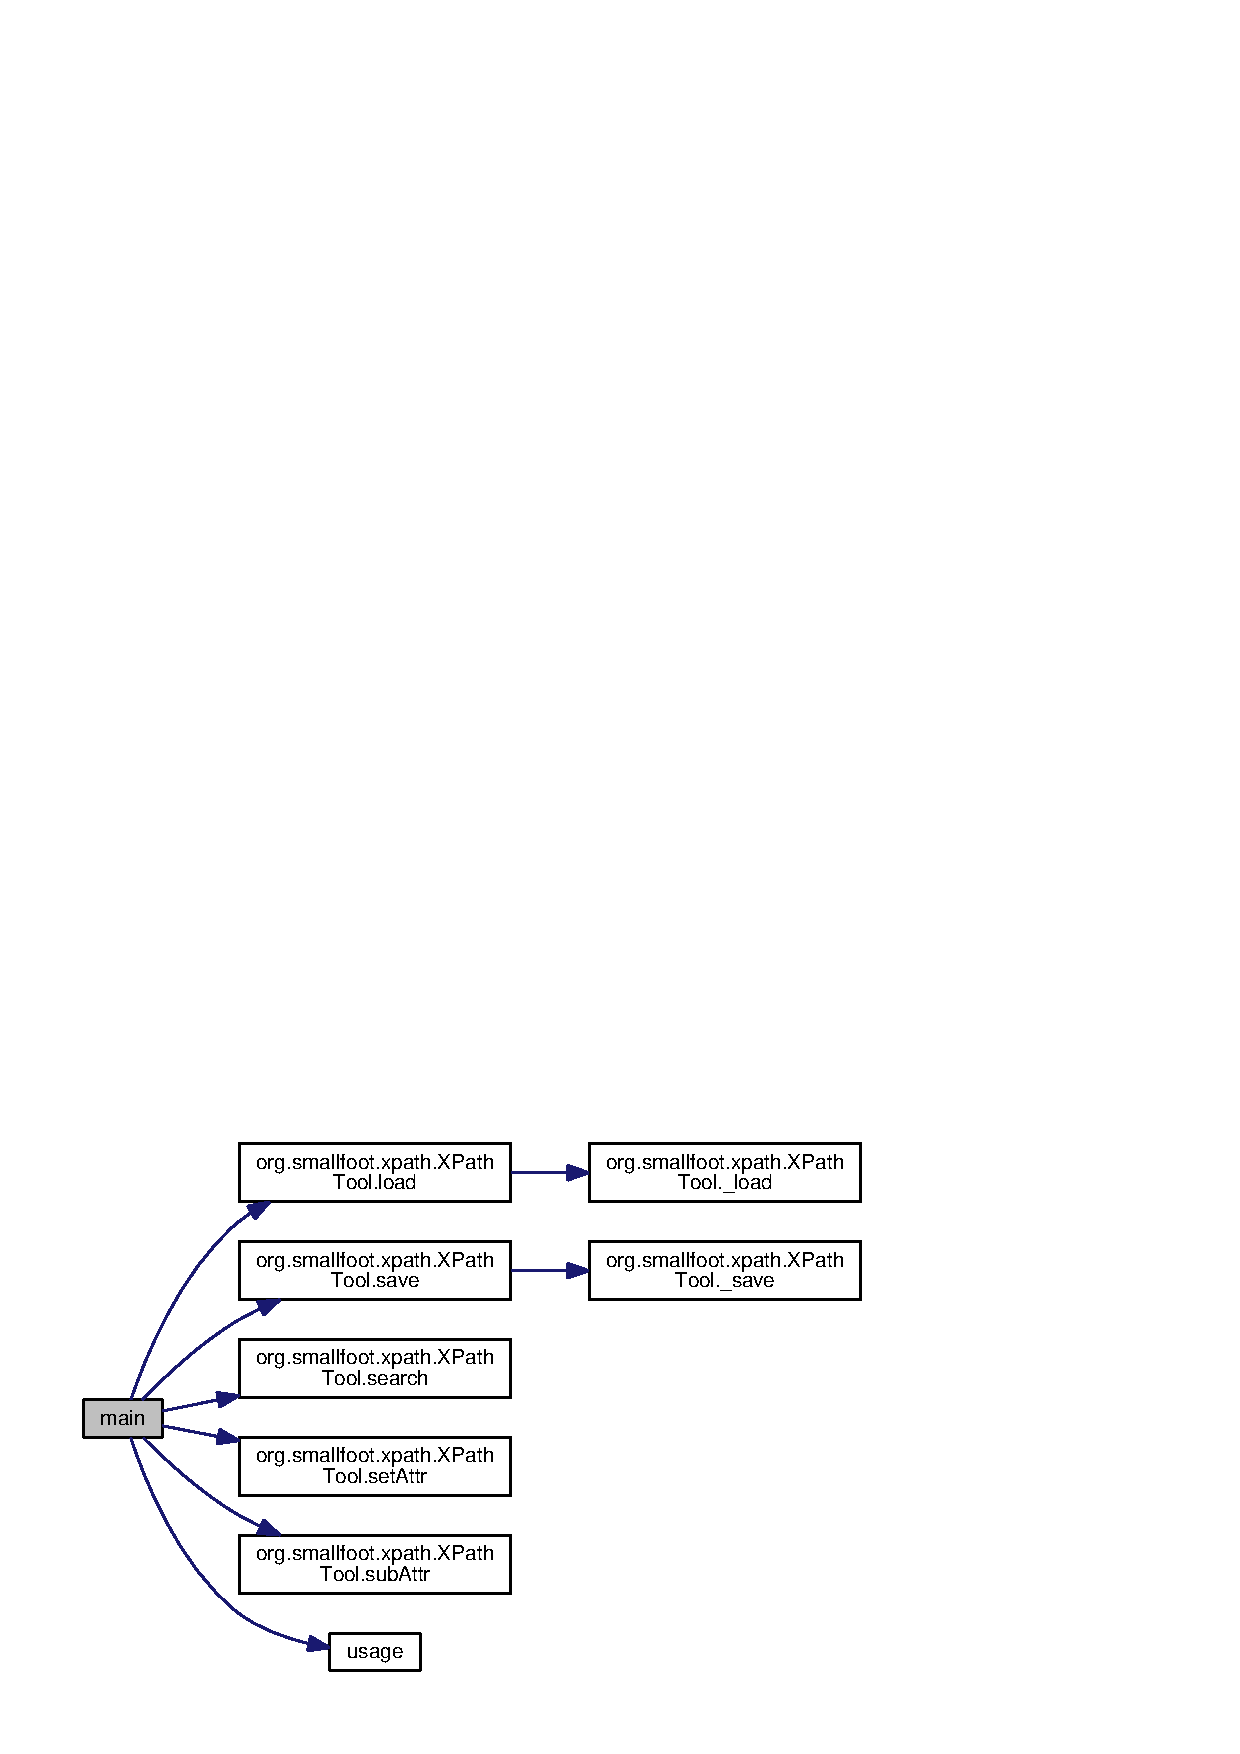
\includegraphics[width=350pt]{classorg_1_1smallfoot_1_1xpath_1_1XPathSet_a8b260eecbaabcef8473fd87ada040682_cgraph}
\end{center}
\end{figure}


\index{org\+::smallfoot\+::xpath\+::\+X\+Path\+Set@{org\+::smallfoot\+::xpath\+::\+X\+Path\+Set}!usage@{usage}}
\index{usage@{usage}!org\+::smallfoot\+::xpath\+::\+X\+Path\+Set@{org\+::smallfoot\+::xpath\+::\+X\+Path\+Set}}
\subsubsection[{usage}]{\setlength{\rightskip}{0pt plus 5cm}static void usage (
\begin{DoxyParamCaption}
\item[{String}]{proc}
\end{DoxyParamCaption}
)\hspace{0.3cm}{\ttfamily [inline]}, {\ttfamily [static]}}\label{classorg_1_1smallfoot_1_1xpath_1_1XPathSet_aec331730d71546f53ebc29753cdfd8a2}


usage messages are useful to those of us with short memories as well (hey, I just need to add swap!) 


\begin{DoxyParams}{Parameters}
{\em proc} & name of the process or program (ie wwndesc) \\
\hline
\end{DoxyParams}


Definition at line 24 of file X\+Path\+Set.\+java.



Referenced by X\+Path\+Set.\+main().



The documentation for this class was generated from the following file\+:\begin{DoxyCompactItemize}
\item 
java/X\+Path\+Set.\+java\end{DoxyCompactItemize}

\section{X\-Path\-Sub Class Reference}
\label{classorg_1_1smallfoot_1_1xpath_1_1XPathSub}\index{X\-Path\-Sub@{X\-Path\-Sub}}


A driving class to interpret commandline arguments and pass them to the underlying \doxyref{X\-Path\-Tool}{p.}{classorg_1_1smallfoot_1_1xpath_1_1XPathTool}.  


\subsection*{Public Member Functions}
\begin{DoxyCompactItemize}
\item 
{\bf X\-Path\-Sub} ()\label{classorg_1_1smallfoot_1_1xpath_1_1XPathSub_aae40faf18a11638688e225f28edd8cf4}

\begin{DoxyCompactList}\small\item\em Class Constructor, uncomplicated. \end{DoxyCompactList}\end{DoxyCompactItemize}
\subsection*{Static Public Member Functions}
\begin{DoxyCompactItemize}
\item 
static void {\bf main} (String[$\,$] args)
\begin{DoxyCompactList}\small\item\em main(args) handles the processing of arguments as sequential actions to pass to the underlying \doxyref{X\-Path\-Tool}{p.}{classorg_1_1smallfoot_1_1xpath_1_1XPathTool}. \end{DoxyCompactList}\end{DoxyCompactItemize}
\subsection*{Private Attributes}
\begin{DoxyCompactItemize}
\item 
int {\bfseries replacements} = 0\label{classorg_1_1smallfoot_1_1xpath_1_1XPathSub_aa0c54debf46b07b29e5d591b260c35f7}

\end{DoxyCompactItemize}


\subsection{Detailed Description}
A driving class to interpret commandline arguments and pass them to the underlying \doxyref{X\-Path\-Tool}{p.}{classorg_1_1smallfoot_1_1xpath_1_1XPathTool}. 

Definition at line 11 of file X\-Path\-Sub.\-java.



\subsection{Member Function Documentation}
\index{org\-::smallfoot\-::xpath\-::\-X\-Path\-Sub@{org\-::smallfoot\-::xpath\-::\-X\-Path\-Sub}!main@{main}}
\index{main@{main}!org::smallfoot::xpath::XPathSub@{org\-::smallfoot\-::xpath\-::\-X\-Path\-Sub}}
\subsubsection[{main}]{\setlength{\rightskip}{0pt plus 5cm}static void main (
\begin{DoxyParamCaption}
\item[{String[$\,$]}]{args}
\end{DoxyParamCaption}
)\hspace{0.3cm}{\ttfamily [inline]}, {\ttfamily [static]}}\label{classorg_1_1smallfoot_1_1xpath_1_1XPathSub_a8b260eecbaabcef8473fd87ada040682}


main(args) handles the processing of arguments as sequential actions to pass to the underlying \doxyref{X\-Path\-Tool}{p.}{classorg_1_1smallfoot_1_1xpath_1_1XPathTool}. 


\begin{DoxyParams}{Parameters}
{\em args} & commandline arguments for processing\-: 
\begin{DoxyItemize}
\item -\/i loads a file (see \doxyref{X\-Path\-Tool\#load(\-String)}{p.}{classorg_1_1smallfoot_1_1xpath_1_1XPathTool_a06e5248d8619f00173d9794f30966dc3} ) 
\item -\/o saves a file (see \doxyref{X\-Path\-Tool\#save(\-String)}{p.}{classorg_1_1smallfoot_1_1xpath_1_1XPathTool_aa9370fe3a8b0b2d5b91a76190c1599e0} ) 
\item -\/r sets a replacement expression\-: anything \char`\"{}found\char`\"{} while running a \char`\"{}-\/f\char`\"{} argument is munged by this value 
\item -\/f starts a search, replacing the value of all matching nodes and attributes with the replcement value given 
\end{DoxyItemize}\\
\hline
\end{DoxyParams}


Definition at line 31 of file X\-Path\-Sub.\-java.



References X\-Path\-Tool.\-search().



Here is the call graph for this function\-:\nopagebreak
\begin{figure}[H]
\begin{center}
\leavevmode
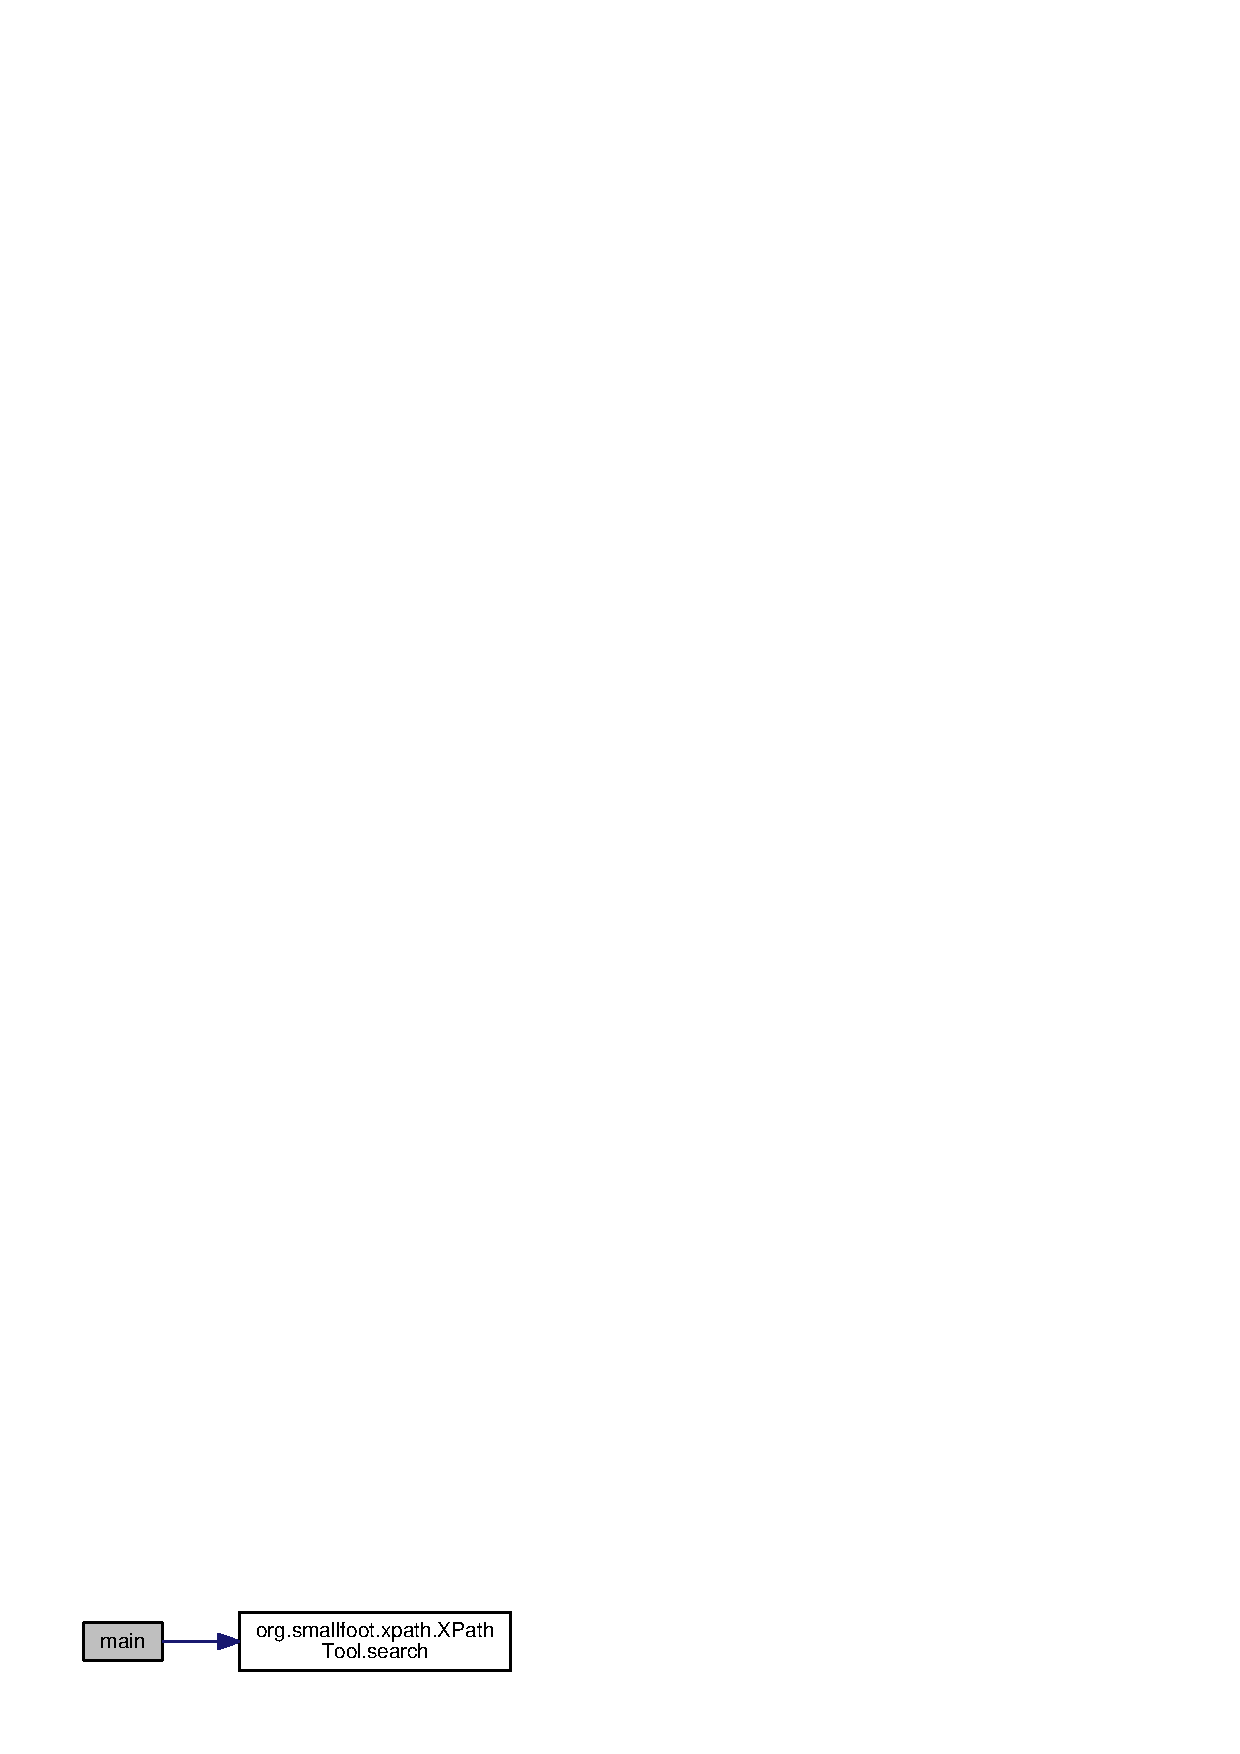
\includegraphics[width=250pt]{classorg_1_1smallfoot_1_1xpath_1_1XPathSub_a8b260eecbaabcef8473fd87ada040682_cgraph}
\end{center}
\end{figure}




The documentation for this class was generated from the following file\-:\begin{DoxyCompactItemize}
\item 
java/X\-Path\-Sub.\-java\end{DoxyCompactItemize}

\section{X\-Path\-Tool Class Reference}
\label{classorg_1_1smallfoot_1_1xpath_1_1XPathTool}\index{X\-Path\-Tool@{X\-Path\-Tool}}


\doxyref{X\-Path\-Tool}{p.}{classorg_1_1smallfoot_1_1xpath_1_1XPathTool} is a relatively uncomplicated wrapper for an X\-Path action\-: it doesn't know what you're doing, and doesn't assume you'll do things in a specific order, but tries to stop you from making really silly errors like saving or searching an unloaded file.  


\subsection*{Public Member Functions}
\begin{DoxyCompactItemize}
\item 
{\bf X\-Path\-Tool} (String xml\-File)
\begin{DoxyCompactList}\small\item\em Class Constructor to create with an initial file to load. \end{DoxyCompactList}\item 
{\bf X\-Path\-Tool} ()\label{classorg_1_1smallfoot_1_1xpath_1_1XPathTool_a78c4db4e609847477447aab80aaa97d6}

\begin{DoxyCompactList}\small\item\em Class Constructor with no initial file. \end{DoxyCompactList}\item 
void {\bf load} (String xml\-File)
\begin{DoxyCompactList}\small\item\em Wrapper to just load the file, spitting out exceptions and stacks as they occur. \end{DoxyCompactList}\item 
void {\bf save} (String out)
\begin{DoxyCompactList}\small\item\em Wrapper to just save the file, spitting out exceptions and stacks as they occur. \end{DoxyCompactList}\item 
Object {\bf search} (String expression, Q\-Name return\-Type)  throws org.\-smallfoot.\-xpath.\-No\-Document\-Exception     
\begin{DoxyCompactList}\small\item\em Search the current X\-M\-L Document for a match, returning a list of matching nodes. \end{DoxyCompactList}\end{DoxyCompactItemize}
\subsection*{Static Public Member Functions}
\begin{DoxyCompactItemize}
\item 
static int {\bf set\-Attr} (Node\-List nodelist, String replacement)
\begin{DoxyCompactList}\small\item\em Consume a list of matches, and for each node (entity or attribute) replace the current value. \end{DoxyCompactList}\item 
static int {\bf sub\-Attr} (Node\-List nodelist, String edit\-Match, String edit\-Replace, boolean global)
\begin{DoxyCompactList}\small\item\em Consume a list of matches, and for each node (entity or attribute) make a Strong.\-replace\-First() or a String.\-replace\-All() \end{DoxyCompactList}\end{DoxyCompactItemize}
\subsection*{Protected Member Functions}
\begin{DoxyCompactItemize}
\item 
void {\bf \-\_\-load} (String xml\-File)  throws javax.\-xml.\-parsers.\-Parser\-Configuration\-Exception, org.\-xml.\-sax.\-S\-A\-X\-Exception, java.\-io.\-I\-O\-Exception     
\begin{DoxyCompactList}\small\item\em Open a file. \end{DoxyCompactList}\item 
void {\bf \-\_\-save} (String xml\-File)  throws javax.\-xml.\-transform.\-Transformer\-Configuration\-Exception, java.\-io.\-File\-Not\-Found\-Exception, javax.\-xml.\-transform.\-Transformer\-Exception, org.\-smallfoot.\-xpath.\-No\-Document\-Exception     
\begin{DoxyCompactList}\small\item\em Save the current X\-M\-L Document to a new file. \end{DoxyCompactList}\end{DoxyCompactItemize}
\subsection*{Private Attributes}
\begin{DoxyCompactItemize}
\item 
org.\-w3c.\-dom.\-Document {\bfseries xml\-Document}\label{classorg_1_1smallfoot_1_1xpath_1_1XPathTool_ad25ef6220eb54575157ab063bc63a0f0}

\end{DoxyCompactItemize}


\subsection{Detailed Description}
\doxyref{X\-Path\-Tool}{p.}{classorg_1_1smallfoot_1_1xpath_1_1XPathTool} is a relatively uncomplicated wrapper for an X\-Path action\-: it doesn't know what you're doing, and doesn't assume you'll do things in a specific order, but tries to stop you from making really silly errors like saving or searching an unloaded file. 

Definition at line 17 of file X\-Path\-Tool.\-java.



\subsection{Constructor \& Destructor Documentation}
\index{org\-::smallfoot\-::xpath\-::\-X\-Path\-Tool@{org\-::smallfoot\-::xpath\-::\-X\-Path\-Tool}!X\-Path\-Tool@{X\-Path\-Tool}}
\index{X\-Path\-Tool@{X\-Path\-Tool}!org::smallfoot::xpath::XPathTool@{org\-::smallfoot\-::xpath\-::\-X\-Path\-Tool}}
\subsubsection[{X\-Path\-Tool}]{\setlength{\rightskip}{0pt plus 5cm}{\bf X\-Path\-Tool} (
\begin{DoxyParamCaption}
\item[{String}]{xml\-File}
\end{DoxyParamCaption}
)\hspace{0.3cm}{\ttfamily [inline]}}\label{classorg_1_1smallfoot_1_1xpath_1_1XPathTool_a8627e2060c614bb6f468d158b66c20b8}


Class Constructor to create with an initial file to load. 


\begin{DoxyParams}{Parameters}
{\em xml\-File} & File to load at start\\
\hline
\end{DoxyParams}
\begin{DoxySeeAlso}{See Also}
\doxyref{load(\-String)}{p.}{classorg_1_1smallfoot_1_1xpath_1_1XPathTool_a06e5248d8619f00173d9794f30966dc3} 
\end{DoxySeeAlso}


Definition at line 28 of file X\-Path\-Tool.\-java.



References X\-Path\-Tool.\-load().



Here is the call graph for this function\-:\nopagebreak
\begin{figure}[H]
\begin{center}
\leavevmode
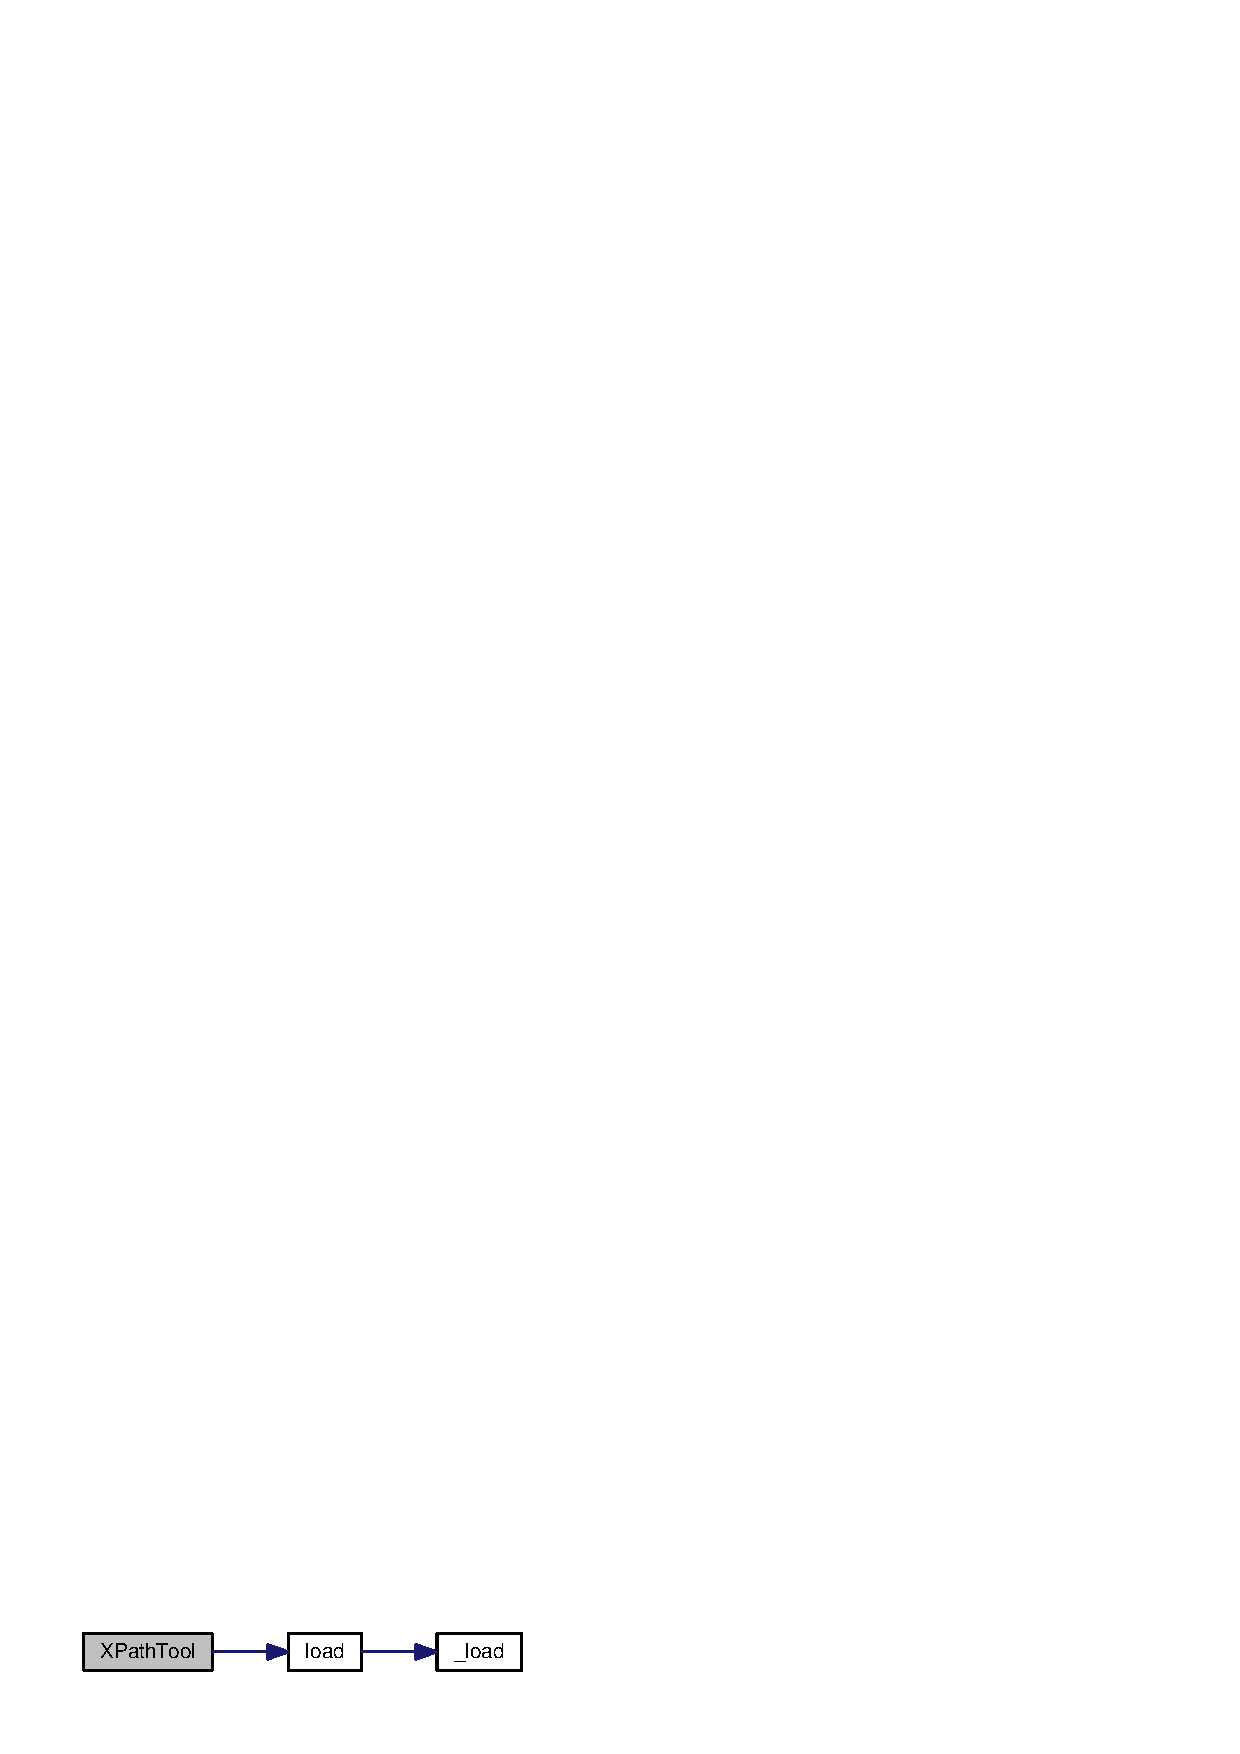
\includegraphics[width=254pt]{classorg_1_1smallfoot_1_1xpath_1_1XPathTool_a8627e2060c614bb6f468d158b66c20b8_cgraph}
\end{center}
\end{figure}




\subsection{Member Function Documentation}
\index{org\-::smallfoot\-::xpath\-::\-X\-Path\-Tool@{org\-::smallfoot\-::xpath\-::\-X\-Path\-Tool}!\-\_\-load@{\-\_\-load}}
\index{\-\_\-load@{\-\_\-load}!org::smallfoot::xpath::XPathTool@{org\-::smallfoot\-::xpath\-::\-X\-Path\-Tool}}
\subsubsection[{\-\_\-load}]{\setlength{\rightskip}{0pt plus 5cm}void \-\_\-load (
\begin{DoxyParamCaption}
\item[{String}]{xml\-File}
\end{DoxyParamCaption}
) throws javax.\-xml.\-parsers.\-Parser\-Configuration\-Exception, org.\-xml.\-sax.\-S\-A\-X\-Exception, java.\-io.\-I\-O\-Exception\hspace{0.3cm}{\ttfamily [inline]}, {\ttfamily [protected]}}\label{classorg_1_1smallfoot_1_1xpath_1_1XPathTool_adc3a8f6eb0246c78615de6cc346d4f99}


Open a file. 

This is actually a wrapper for the complex usage of javax.\-xml.\-parsers.\-Document\-Builder\-Factory to find a singleton to instantiate a document from a file.


\begin{DoxyParams}{Parameters}
{\em xml\-File} & file to load \\
\hline
\end{DoxyParams}

\begin{DoxyExceptions}{Exceptions}
{\em java.\-io.\-I\-O\-Exception} & on issues loading the file given as a parameter \\
\hline
{\em javax.\-xml.\-parsers.\-Parser\-Configuration\-Exception} & when the javax.\-xml.\-parsers.\-Document\-Builder\-Factory is butchered \\
\hline
{\em org.\-xml.\-sax.\-S\-A\-X\-Exception} & on parsing issues \\
\hline
\end{DoxyExceptions}


Definition at line 50 of file X\-Path\-Tool.\-java.



Referenced by X\-Path\-Tool.\-load().

\index{org\-::smallfoot\-::xpath\-::\-X\-Path\-Tool@{org\-::smallfoot\-::xpath\-::\-X\-Path\-Tool}!\-\_\-save@{\-\_\-save}}
\index{\-\_\-save@{\-\_\-save}!org::smallfoot::xpath::XPathTool@{org\-::smallfoot\-::xpath\-::\-X\-Path\-Tool}}
\subsubsection[{\-\_\-save}]{\setlength{\rightskip}{0pt plus 5cm}void \-\_\-save (
\begin{DoxyParamCaption}
\item[{String}]{xml\-File}
\end{DoxyParamCaption}
) throws javax.\-xml.\-transform.\-Transformer\-Configuration\-Exception, java.\-io.\-File\-Not\-Found\-Exception, javax.\-xml.\-transform.\-Transformer\-Exception, {\bf org.\-smallfoot.\-xpath.\-No\-Document\-Exception}\hspace{0.3cm}{\ttfamily [inline]}, {\ttfamily [protected]}}\label{classorg_1_1smallfoot_1_1xpath_1_1XPathTool_adb7f600accd4a29f376ce8e52edff11a}


Save the current X\-M\-L Document to a new file. 

based partially on {\tt Document\-Builder\-Factory.\-java} and influenced by {\tt Writing X\-M\-L on Android}


\begin{DoxyParams}{Parameters}
{\em xml\-File} & filename to save into \\
\hline
\end{DoxyParams}

\begin{DoxyExceptions}{Exceptions}
{\em java.\-io.\-File\-Not\-Found\-Exception} & on issues creating the output filestream on xml\-File (ie missing interposing directory or permissions) \\
\hline
{\em javax.\-xml.\-transform.\-Transformer\-Configuration\-Exception} & when the javax.\-xml.\-transform.\-Transformer\-Factory is butchered \\
\hline
{\em javax.\-xml.\-transform.\-Transformer\-Exception} & for exceptions on the final step, the transformation itself \\
\hline
{\em \doxyref{org.\-smallfoot.\-xpath.\-No\-Document\-Exception}{p.}{classorg_1_1smallfoot_1_1xpath_1_1NoDocumentException}} & if the user has tried to search before a document is loaded \\
\hline
\end{DoxyExceptions}


Definition at line 87 of file X\-Path\-Tool.\-java.



Referenced by X\-Path\-Tool.\-save().

\index{org\-::smallfoot\-::xpath\-::\-X\-Path\-Tool@{org\-::smallfoot\-::xpath\-::\-X\-Path\-Tool}!load@{load}}
\index{load@{load}!org::smallfoot::xpath::XPathTool@{org\-::smallfoot\-::xpath\-::\-X\-Path\-Tool}}
\subsubsection[{load}]{\setlength{\rightskip}{0pt plus 5cm}void load (
\begin{DoxyParamCaption}
\item[{String}]{xml\-File}
\end{DoxyParamCaption}
)\hspace{0.3cm}{\ttfamily [inline]}}\label{classorg_1_1smallfoot_1_1xpath_1_1XPathTool_a06e5248d8619f00173d9794f30966dc3}


Wrapper to just load the file, spitting out exceptions and stacks as they occur. 


\begin{DoxyParams}{Parameters}
{\em xml\-File} & file to load \\
\hline
\end{DoxyParams}


Definition at line 61 of file X\-Path\-Tool.\-java.



References X\-Path\-Tool.\-\_\-load().



Referenced by X\-Path\-Tool.\-X\-Path\-Tool().



Here is the call graph for this function\-:\nopagebreak
\begin{figure}[H]
\begin{center}
\leavevmode
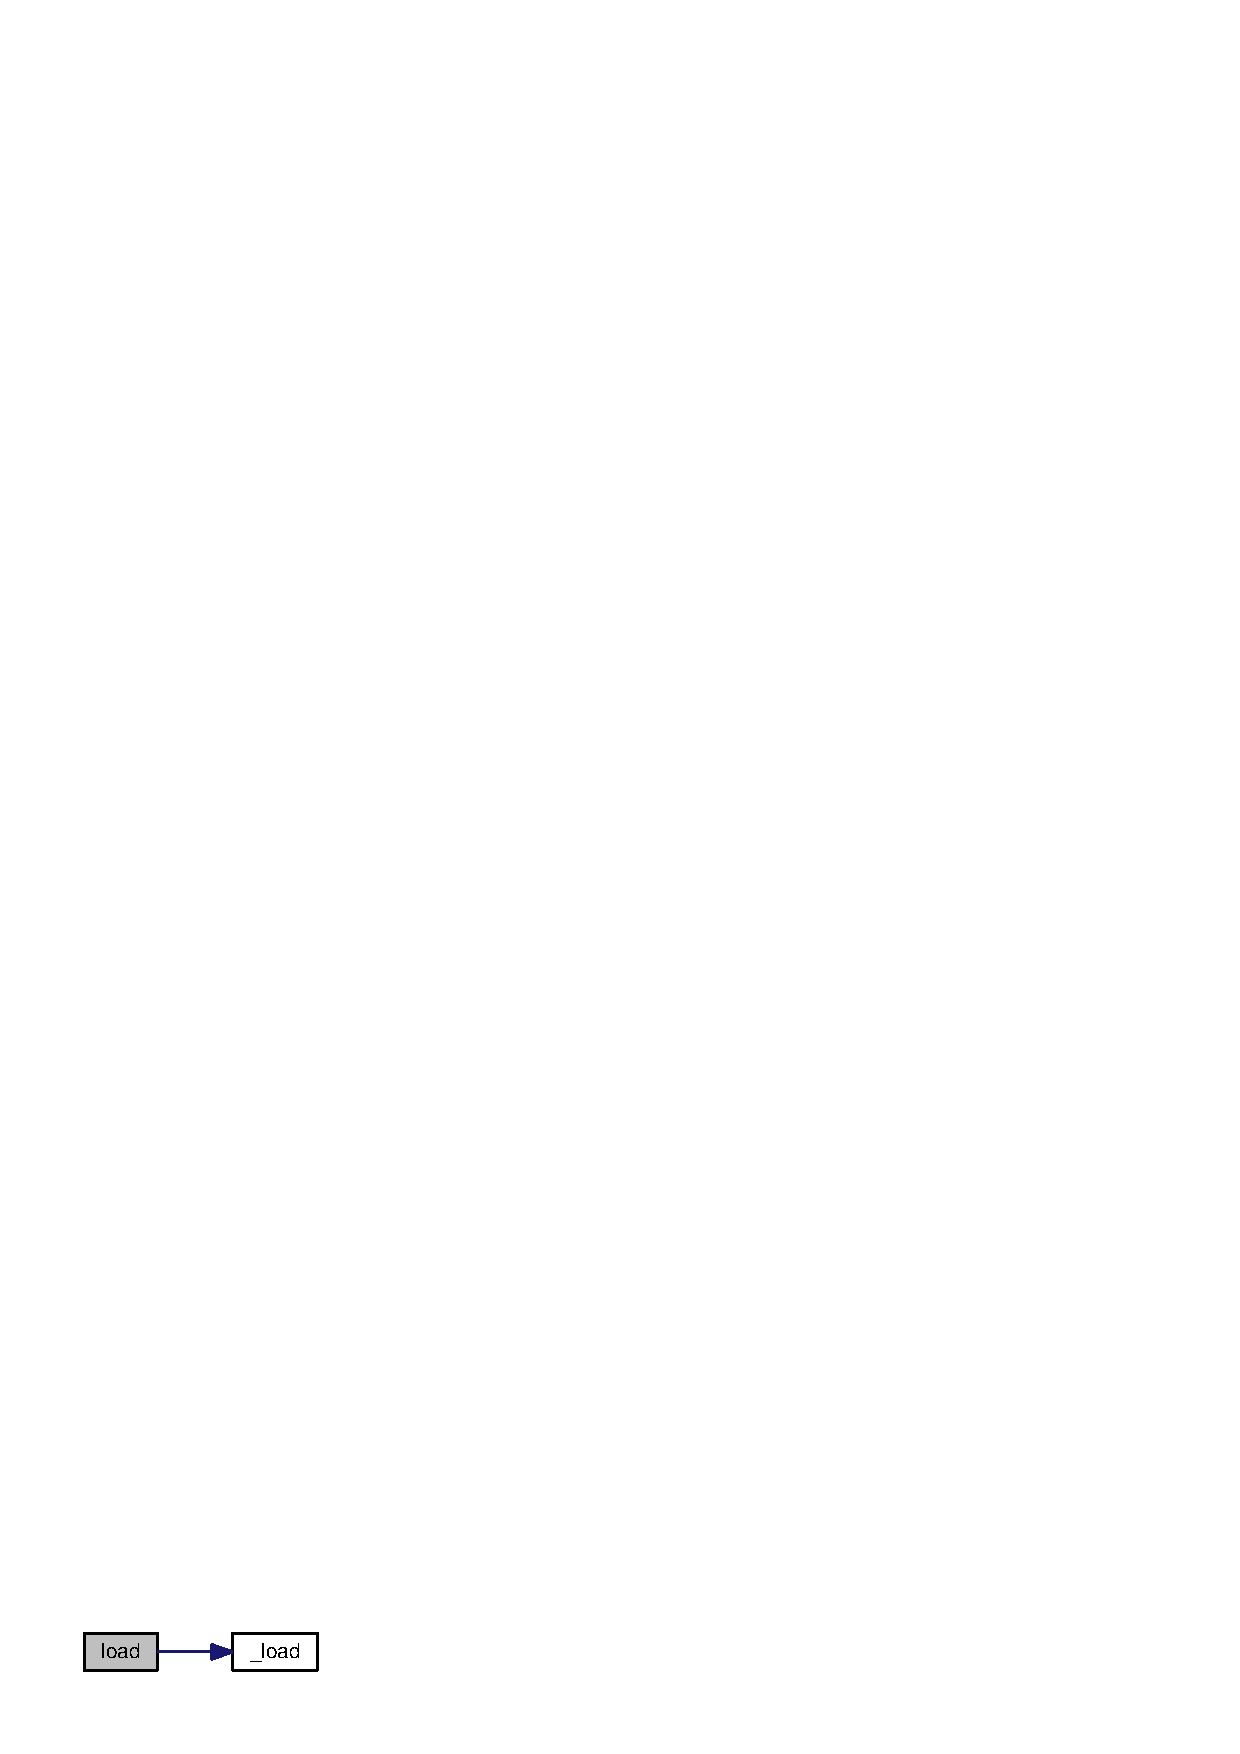
\includegraphics[width=156pt]{classorg_1_1smallfoot_1_1xpath_1_1XPathTool_a06e5248d8619f00173d9794f30966dc3_cgraph}
\end{center}
\end{figure}


\index{org\-::smallfoot\-::xpath\-::\-X\-Path\-Tool@{org\-::smallfoot\-::xpath\-::\-X\-Path\-Tool}!save@{save}}
\index{save@{save}!org::smallfoot::xpath::XPathTool@{org\-::smallfoot\-::xpath\-::\-X\-Path\-Tool}}
\subsubsection[{save}]{\setlength{\rightskip}{0pt plus 5cm}void save (
\begin{DoxyParamCaption}
\item[{String}]{out}
\end{DoxyParamCaption}
)\hspace{0.3cm}{\ttfamily [inline]}}\label{classorg_1_1smallfoot_1_1xpath_1_1XPathTool_aa9370fe3a8b0b2d5b91a76190c1599e0}


Wrapper to just save the file, spitting out exceptions and stacks as they occur. 


\begin{DoxyParams}{Parameters}
{\em out} & filename to save into \\
\hline
\end{DoxyParams}


Definition at line 106 of file X\-Path\-Tool.\-java.



References X\-Path\-Tool.\-\_\-save().



Here is the call graph for this function\-:\nopagebreak
\begin{figure}[H]
\begin{center}
\leavevmode
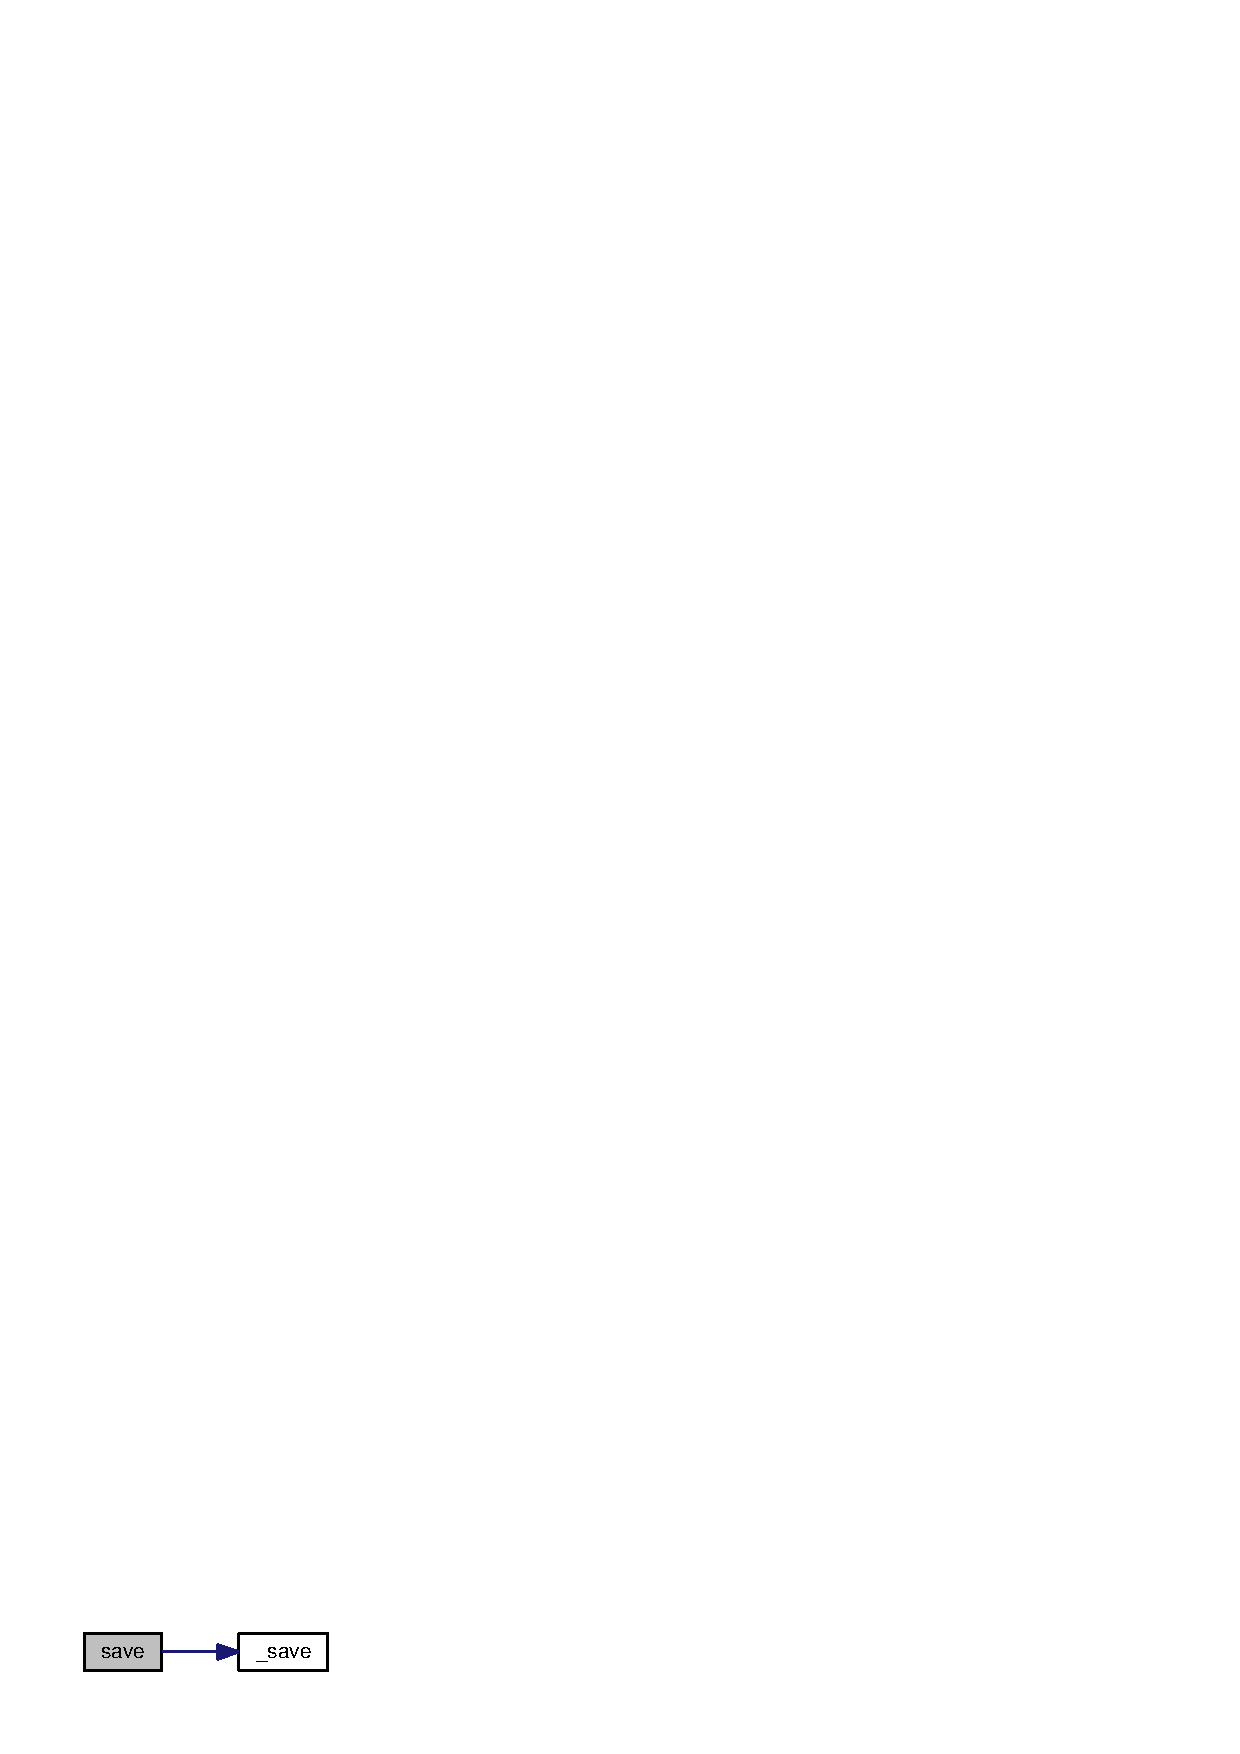
\includegraphics[width=162pt]{classorg_1_1smallfoot_1_1xpath_1_1XPathTool_aa9370fe3a8b0b2d5b91a76190c1599e0_cgraph}
\end{center}
\end{figure}


\index{org\-::smallfoot\-::xpath\-::\-X\-Path\-Tool@{org\-::smallfoot\-::xpath\-::\-X\-Path\-Tool}!search@{search}}
\index{search@{search}!org::smallfoot::xpath::XPathTool@{org\-::smallfoot\-::xpath\-::\-X\-Path\-Tool}}
\subsubsection[{search}]{\setlength{\rightskip}{0pt plus 5cm}Object search (
\begin{DoxyParamCaption}
\item[{String}]{expression, }
\item[{Q\-Name}]{return\-Type}
\end{DoxyParamCaption}
) throws {\bf org.\-smallfoot.\-xpath.\-No\-Document\-Exception}\hspace{0.3cm}{\ttfamily [inline]}}\label{classorg_1_1smallfoot_1_1xpath_1_1XPathTool_af1af4b7f062c6dd322b7e7a81209afb6}


Search the current X\-M\-L Document for a match, returning a list of matching nodes. 


\begin{DoxyParams}{Parameters}
{\em expression} & X\-Path expression to search for \\
\hline
{\em return\-Type} & namespace context against which the expression is evaluated \\
\hline
\end{DoxyParams}

\begin{DoxyExceptions}{Exceptions}
{\em \doxyref{org.\-smallfoot.\-xpath.\-No\-Document\-Exception}{p.}{classorg_1_1smallfoot_1_1xpath_1_1NoDocumentException}} & if the user has tried to search before a document is loaded \\
\hline
\end{DoxyExceptions}


Definition at line 129 of file X\-Path\-Tool.\-java.



Referenced by X\-Path\-Sub.\-main(), and X\-Path\-Set.\-main().

\index{org\-::smallfoot\-::xpath\-::\-X\-Path\-Tool@{org\-::smallfoot\-::xpath\-::\-X\-Path\-Tool}!set\-Attr@{set\-Attr}}
\index{set\-Attr@{set\-Attr}!org::smallfoot::xpath::XPathTool@{org\-::smallfoot\-::xpath\-::\-X\-Path\-Tool}}
\subsubsection[{set\-Attr}]{\setlength{\rightskip}{0pt plus 5cm}static int set\-Attr (
\begin{DoxyParamCaption}
\item[{Node\-List}]{nodelist, }
\item[{String}]{replacement}
\end{DoxyParamCaption}
)\hspace{0.3cm}{\ttfamily [inline]}, {\ttfamily [static]}}\label{classorg_1_1smallfoot_1_1xpath_1_1XPathTool_aef43485334ab87e6db498fe403162255}


Consume a list of matches, and for each node (entity or attribute) replace the current value. 

This function allows specific programmatic replacement of string values in X\-M\-L to reduce the chance of user error and typos creating erroneous X\-M\-L.


\begin{DoxyParams}{Parameters}
{\em nodelist} & list of nodes containing targets/matches to alter \\
\hline
{\em replacement} & string to replace for matches \\
\hline
\end{DoxyParams}
\begin{DoxyReturn}{Returns}
number of matches made 
\end{DoxyReturn}


Definition at line 202 of file X\-Path\-Tool.\-java.

\index{org\-::smallfoot\-::xpath\-::\-X\-Path\-Tool@{org\-::smallfoot\-::xpath\-::\-X\-Path\-Tool}!sub\-Attr@{sub\-Attr}}
\index{sub\-Attr@{sub\-Attr}!org::smallfoot::xpath::XPathTool@{org\-::smallfoot\-::xpath\-::\-X\-Path\-Tool}}
\subsubsection[{sub\-Attr}]{\setlength{\rightskip}{0pt plus 5cm}static int sub\-Attr (
\begin{DoxyParamCaption}
\item[{Node\-List}]{nodelist, }
\item[{String}]{edit\-Match, }
\item[{String}]{edit\-Replace, }
\item[{boolean}]{global}
\end{DoxyParamCaption}
)\hspace{0.3cm}{\ttfamily [inline]}, {\ttfamily [static]}}\label{classorg_1_1smallfoot_1_1xpath_1_1XPathTool_a2e34675797f629121c1b2a74a19ebd34}


Consume a list of matches, and for each node (entity or attribute) make a Strong.\-replace\-First() or a String.\-replace\-All() 

This function is added as a convenience function to allow semi-\/contextual replacement of strings when converting other X\-M\-L content -- this allows single atomic commands to rename components to avoid name-\/clashes and unintended replacements.


\begin{DoxyParams}{Parameters}
{\em nodelist} & list of nodes containing targets/matches to alter \\
\hline
{\em edit\-Match} & string to match for replacement \\
\hline
{\em edit\-Replace} & string to replace for matches \\
\hline
{\em global} & whether to replace globally (like sed -\/e 's/\-X/y/g' -- the 'g' at the end) -- which is whether to use a Strong.\-replace\-First() or a String.\-replace\-All() \\
\hline
\end{DoxyParams}
\begin{DoxyReturn}{Returns}
number of matches made 
\end{DoxyReturn}


Definition at line 158 of file X\-Path\-Tool.\-java.



The documentation for this class was generated from the following file\-:\begin{DoxyCompactItemize}
\item 
java/X\-Path\-Tool.\-java\end{DoxyCompactItemize}

%--- End generated contents ---

% Index
\newpage
\phantomsection
\addcontentsline{toc}{chapter}{Index}
\printindex

\end{document}
